\section{障碍法}
% Source PDF page 582 (printed p. 568), section 11.3 begins here.
我们已经看到，点 $x^\star(t)$ 的次优程度为 $m/t$，对偶可行点对 $\lambda^\star(t),\nu^\star(t)$ 为这一精度提供了证书。由此得到一种非常直接的方法，可以按指定精度 $\epsilon$ 求解原问题 (11.1)：取 $t=m/\epsilon$，并用牛顿法求解等式约束问题
% Source PDF page 583 (printed p. 569)
\[
\begin{aligned}
\text{最小化}\quad&(m/\epsilon)f_0(x)+\phi(x)\\
\text{约束为}\quad&Ax=b.
\end{aligned}
\]
这种方法可以称为无约束最小化法，因为它通过求解一个无约束或线性约束问题，就能按保证的精度求解不等式约束问题 (11.1)。尽管对于小问题、好的初始点和中等精度（即 $\epsilon$ 不太小），这种方法能够很好地工作，但在其他情况下效果不好。因此，它极少被采用，甚至从未被采用。

\subsection{障碍法}
对无约束最小化法作一个简单扩展，就能得到效果很好的方法。它依次求解一系列无约束（或线性约束）最小化问题，以上一次找到的点作为下一个无约束最小化问题的初始点。换言之，对一系列递增的 $t$ 值计算 $x^\star(t)$，直至 $t\ge m/\epsilon$，从而保证得到原问题的一个 $\epsilon$ 次优解。Fiacco 和 McCormick 在20世纪60年代首次提出这种方法时，将其称为序列无约束最小化技术（SUMT）。现在通常称为\emph{障碍法}或\emph{路径跟踪法}。它的一个简单版本如下。

\begin{origalgorithm}{11.1}
\textbf{障碍法。}

给定严格可行点 $x$，$t:=t^{(0)}>0$，$\mu>1$，容差 $\epsilon>0$。

重复：
\begin{enumerate}
\item \textbf{中心化步骤。} 以 $x$ 为起点，在 $Ax=b$ 约束下最小化 $tf_0+\phi$，计算 $x^\star(t)$。
\item \textbf{更新。} $x:=x^\star(t)$。
\item \textbf{停止准则。} 若 $m/t<\epsilon$，退出。
\item \textbf{增大 $t$。} $t:=\mu t$。
\end{enumerate}
\end{origalgorithm}
除第一次迭代外，每次迭代均以前一次计算的中心点为起点，计算中心点 $x^\star(t)$，随后将 $t$ 乘以因子 $\mu>1$。算法还可返回 $\lambda=\lambda^\star(t)$、$\nu=\nu^\star(t)$，即一个对偶 $\epsilon$ 次优点，也就是 $x$ 的证书。

每执行一次第1步，称为一次\emph{中心化步骤}（因为在计算中心点）或\emph{外迭代}；第一次中心化步骤，即计算 $x^\star(t^{(0)})$，称为\emph{初始中心化步骤}。（因此，取 $t^{(0)}=m/\epsilon$ 的简单算法只有初始中心化步骤。）第1步可以使用任意线性约束最小化方法，但我们将假设使用牛顿法。中心化步骤中的牛顿迭代或牛顿步称为\emph{内迭代}。每个内迭代步均有一个原始可行点；但只有在每次外迭代（中心化）结束时，才有对偶可行点。

% Source PDF page 584 (printed p. 570)
\subsubsection*{中心化的精度}
对中心化问题的求解精度，有几点需要说明。没有必要精确计算 $x^\star(t)$，因为中心路径本身的意义只在于：当 $t\to\infty$ 时，它引向原问题的解；非精确中心化仍会产生收敛到最优点的点列 $x^{(k)}$。然而，非精确中心化意味着由 (11.10) 计算出的 $\lambda^\star(t),\nu^\star(t)$ 并非精确对偶可行。可以给公式 (11.10) 加一个修正项来解决这个问题：只要计算出的 $x$ 接近中心路径，即接近 $x^\star(t)$，便能得到对偶可行点（见习题11.9）。另一方面，与计算 $tf_0+\phi$ 的一个较好最小化点相比，计算一个极高精度最小化点的额外成本很少，至多增加几个牛顿步。因此，假设精确中心化并非不合理。

\subsubsection*{$\mu$ 的选择}
参数 $\mu$ 的选择涉及内迭代次数和外迭代次数之间的权衡。当 $\mu$ 很小（即接近 $1$）时，每次外迭代只将 $t$ 增大一个较小倍数。因此，牛顿过程的初始点，也就是前一个迭代点 $x$，是很好的起点，计算下一迭代点所需的牛顿步很少。于是，小 $\mu$ 对应每次外迭代较少的牛顿步，但由于每次外迭代只把间隙减小很少，外迭代次数就会很多。这种情况下，迭代点（实际上也包括内迭代的迭代点）会紧贴中心路径，这也解释了“路径跟踪法”这个名称。

当 $\mu$ 很大时，情况相反。每次外迭代后 $t$ 大幅增加，当前迭代点通常不再是下一迭代点的良好近似，所以内迭代次数会多得多。这样“激进”地更新 $t$，会减少外迭代次数，因为每次外迭代都使对偶间隙缩小 $\mu$ 倍，但会增加内迭代次数。$\mu$ 很大时，中心路径上的迭代点相距很远，内迭代点会大幅偏离中心路径。

实践与理论都证实了选择 $\mu$ 时的这一权衡。在实践中，小 $\mu$（接近 $1$）导致很多次外迭代，每次仅有几个牛顿步。在相当宽的范围内，例如 $\mu$ 从约 $3$ 到约 $100$，这两种效应几乎相抵，总牛顿步数近似不变。这说明 $\mu$ 的选择并不特别关键，约 $10$ 至 $20$ 的值似乎效果不错。当按最好的最坏情况总牛顿步数上界来选择 $\mu$ 时，则采用接近 $1$ 的值。

\subsubsection*{$t^{(0)}$ 的选择}
另一个重要问题是 $t$ 初值的选择。这里的权衡很简单：若 $t^{(0)}$ 太大，第一次外迭代需要过多内迭代；若 $t^{(0)}$ 太小，算法需要额外的外迭代，第一次中心化中也可能有过多内迭代。

由于 $m/t^{(0)}$ 是初始中心化结束时得到的对偶间隙，
% Source PDF page 585 (printed p. 571)
一个合理选择是使 $m/t^{(0)}$ 大约与 $f_0(x^{(0)})-p^\star$ 同阶，或是它的 $\mu$ 倍。例如，若已知一个对偶可行点 $\lambda,\nu$，其对偶间隙为 $\eta=f_0(x^{(0)})-g(\lambda,\nu)$，则可取 $t^{(0)}=m/\eta$。这样，第一次外迭代只是计算一个点对，其对偶间隙与初始原始、对偶可行点的间隙相同。

中心路径条件 (11.7) 还提示了另一种可能。把
\begin{equation}
\inf_\nu\norm{t\nabla f_0(x^{(0)})+\nabla\phi(x^{(0)})+A^\T\nu}_2\tag{11.12}
\end{equation}
解释为 $x^{(0)}$ 偏离 $x^\star(t)$ 的程度，并将使 (11.12) 最小的 $t$ 值作为 $t^{(0)}$。（这个 $t$ 和 $\nu$ 可以通过求解最小二乘问题得到。）

这一方法的一个变体，是用 $x$ 与 $x^\star(t)$ 之间仿射不变的偏离度量代替欧氏范数。选择使下式最小的 $t$ 和 $\nu$：
\begin{align*}
\alpha(t,\nu)={}&\bigl(t\nabla f_0(x^{(0)})+\nabla\phi(x^{(0)})+A^\T\nu\bigr)^\T H_0^{-1}\\
&\qquad\bigl(t\nabla f_0(x^{(0)})+\nabla\phi(x^{(0)})+A^\T\nu\bigr),
\end{align*}
其中
\[
H_0=t\nabla^2 f_0(x^{(0)})+\nabla^2\phi(x^{(0)}).
\]
（可以证明，$\inf_\nu\alpha(t,\nu)$ 是 $tf_0+\phi$ 在 $x^{(0)}$ 处的牛顿减量的平方。）由于 $\alpha$ 是关于 $\nu$ 和 $t$ 的二次除以线性函数，它为凸函数。

\subsubsection*{不可行初始点牛顿法}
障碍法的一种变体使用不可行初始点牛顿法（见第10.3节）完成中心化。因此，障碍法的初始点 $x^{(0)}$ 满足 $x^{(0)}\in\dom f_0$，且 $f_i(x^{(0)})<0$，$i=1,\ldots,m$，但不一定满足 $Ax^{(0)}=b$。假设问题严格可行，则第一次中心化中某一步会接受完整牛顿步，此后所有迭代点均原始可行，算法与标准障碍法一致。

\subsection{例子}
\subsubsection*{不等式形式的线性规划}
第一个例子是一个小型不等式形式 LP，
\[
\begin{aligned}\text{最小化}\quad&c^\T x\\\text{约束为}\quad&Ax\preceq b,\end{aligned}
\]
其中 $A\in\R^{100\times50}$。随机生成数据，使问题严格原始可行、严格对偶可行，而且最优值 $p^\star=1$。

初始点 $x^{(0)}$ 在中心路径上，对偶间隙为 $100$。用障碍法求解，对偶间隙小于 $10^{-6}$ 时终止。用带回溯的牛顿法求解中心化问题，参数为 $\alpha=0.01$、$\beta=0.5$。
% Source PDF page 586 (printed p. 572)
牛顿法的停止准则为 $\lambda(x)^2/2\le10^{-5}$，其中 $\lambda(x)$ 是函数 $tc^\T x+\phi(x)$ 的牛顿减量。

\begin{figure}[htbp]\centering
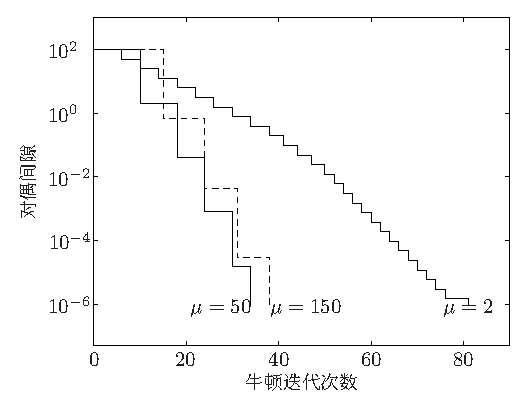
\includegraphics[width=.65\textwidth]{figures/ch11-04.pdf}
\caption*{图11.4 小型 LP 的障碍法求解过程：对偶间隙与累计牛顿步数的关系。三条曲线分别对应参数 $\mu=2,50,150$。各情况下，对偶间隙都近似线性收敛。}
\end{figure}
图11.4展示了三个参数 $\mu$ 值对应的障碍法进展。纵轴以对数尺度表示对偶间隙，横轴为累计内迭代次数，即牛顿步数，这是计算工作量的自然度量。每条曲线呈阶梯形，每个台阶对应一次外迭代。每段水平阶面的宽度，就是该次外迭代所需的牛顿步数。每段竖直阶面的高度恰好对应因子 $\mu$，因为每次外迭代结束时，对偶间隙都缩小 $\mu$ 倍。

这些曲线展示了障碍法的几个典型特征。首先，该方法效果很好，对偶间隙近似线性收敛。这是因为，对每个 $\mu$ 值，重新中心化所需的牛顿步数近似不变。$\mu=50$ 和 $\mu=150$ 时，障碍法求解该问题的总牛顿步数在 $35$ 至 $40$ 之间。

图11.4清楚地显示出 $\mu$ 选择中的权衡。$\mu=2$ 时，阶面较短，重新中心化约需 $2$ 或 $3$ 个牛顿步；但竖直阶面也短，因为每次外迭代只把对偶间隙缩小 $2$ 倍。另一个极端是 $\mu=150$，水平阶面较长，通常约需 $7$ 个牛顿步，但竖直阶面也大得多，因为每次外迭代都使对偶间隙缩小 $150$ 倍。

图11.5进一步考察选择 $\mu$ 的权衡。取 $1.2$ 至 $200$ 之间的 $25$ 个 $\mu$ 值，用障碍法求解该 LP，当对偶间隙小于 $10^{-3}$ 时终止。图中绘出了求解所需总牛顿步数随参数 $\mu$ 的变化。
% Source PDF page 587 (printed p. 573)
\begin{figure}[htbp]\centering
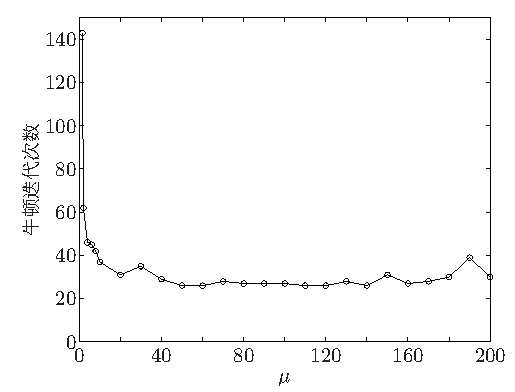
\includegraphics[width=.65\textwidth]{figures/ch11-05.pdf}
\caption*{图11.5 小型 LP 中参数 $\mu$ 的选择权衡。纵轴为将对偶间隙从 $100$ 减小到 $10^{-3}$ 所需的总牛顿步数，横轴为 $\mu$。图中可见，$\mu$ 大于约 $3$ 时障碍法效果很好，而对 $\mu$ 的具体数值并不敏感。}
\end{figure}
从图中可见，当 $\mu$ 处于约 $3$ 至 $200$ 的宽范围内时，障碍法表现都很好。正如直观所预期，$\mu$ 过小时，需要更多次外迭代，总牛顿步数因而上升。一个有意思的观察是，$\mu$ 大于约 $3$ 时，总牛顿步数变化不大。因此，当 $\mu$ 在这个范围内增大时，外迭代次数减少，恰好被每次外迭代所需牛顿步数的增加抵消。$\mu$ 进一步增大时，障碍法的性能变得较难预测，即更依赖具体问题实例。由于增大 $\mu$ 不再改善性能，选择 $10$ 至 $100$ 范围内的值比较合适。

\subsubsection*{几何规划}
考虑凸形式的几何规划，
\[
\begin{aligned}
\text{最小化}\quad&\log\left(\sum_{k=1}^{K_0}\exp(a_{0k}^\T x+b_{0k})\right)\\
\text{约束为}\quad&\log\left(\sum_{k=1}^{K_i}\exp(a_{ik}^\T x+b_{ik})\right)\le0,\quad i=1,\ldots,m,
\end{aligned}
\]
变量为 $x\in\R^n$，相应的对数障碍为
\[
\phi(x)=-\sum_{i=1}^m\log\left(-\log\sum_{k=1}^{K_i}\exp(a_{ik}^\T x+b_{ik})\right).
\]
所考察的实例有 $n=50$ 个变量和 $m=100$ 个不等式，与上面的小型 LP 相同。目标函数和各个约束函数都包含
% Source PDF page 588 (printed p. 574)
$K_i=5$ 项。随机生成这个实例，使其严格原始可行、严格对偶可行，而且最优值为 $1$。

\begin{figure}[htbp]\centering
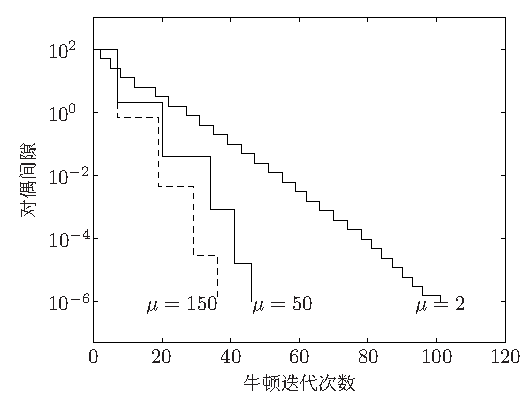
\includegraphics[width=.65\textwidth]{figures/ch11-06.pdf}
\caption*{图11.6 小型 GP 的障碍法求解过程：对偶间隙与累计牛顿步数的关系。这里同样可见对偶间隙近似线性收敛。}
\end{figure}
初始点 $x^{(0)}$ 位于中心路径上，对偶间隙为 $100$。分别取 $\mu=2$、$\mu=50$、$\mu=150$，用障碍法求解，当对偶间隙小于 $10^{-6}$ 时终止。中心化问题用牛顿法求解，参数与 LP 例子相同，即 $\alpha=0.01$、$\beta=0.5$，停止准则为 $\lambda(x)^2/2\le10^{-5}$。

图11.6给出了对偶间隙随累计牛顿步数的变化，它与图11.4中的 LP 曲线非常相似。特别地，每次中心化所需的牛顿步数近似不变，因此对偶间隙近似线性收敛。

求解所需总牛顿步数随参数 $\mu$ 的变化，也与 LP 例子十分相似。对于这个 GP，$\mu$ 在 $10$ 至 $200$ 之间时，将对偶间隙减小到 $10^{-3}$ 以下约需 $30$ 个牛顿步，实际范围约为 $20$ 至 $40$。所以这里选择 $10$ 至 $100$ 范围内的 $\mu$ 也比较合适。

\subsubsection*{一族标准形式 LP}
在上面的例子中，我们对维数相近的随机 LP 和 GP 实例，考察了障碍法进展，即对偶间隙随累计牛顿步数的变化。两者的结果非常相似，都显示出对偶间隙随牛顿步数近似线性收敛。还考察了性能随参数 $\mu$ 的变化，两个例子的结果也基本相同。$\mu$ 大于约 $10$ 时，障碍法效果很好，约需 $30$ 个牛顿步就能将对偶间隙从 $10^2$ 减小到 $10^{-6}$。
% Source PDF page 589 (printed p. 575)
在两种情况下，只要 $\mu$ 大于约 $10$，其选择几乎不影响所需的总牛顿步数。

本节考察障碍法性能随问题维数的变化。考虑标准形式 LP
\[
\begin{aligned}
\text{最小化}\quad&c^\T x\\\text{约束为}\quad&Ax=b,\qquad x\succeq0,
\end{aligned}
\]
其中 $A\in\R^{m\times n}$。对一族随机生成的实例，研究所需总牛顿步数与变量数 $n$、等式约束数 $m$ 的关系。取 $n=2m$，即变量数为约束数的两倍。

问题按如下方式生成。$A$ 的元素独立同分布，服从均值为零、方差为一的正态分布 $\mathcal N(0,1)$。取 $b=Ax^{(0)}$，其中 $x^{(0)}$ 各分量独立，均匀分布在 $[0,1]$ 上。这保证问题严格原始可行，因为 $x^{(0)}\succ0$ 且可行。构造成本向量 $c$ 时，先计算向量 $z\in\R^m$ 和 $s\in\R^n$，前者各分量服从 $\mathcal N(0,1)$，后者各分量均匀分布在 $[0,1]$ 上，然后取 $c=A^\T z+s$。这保证问题严格对偶可行，因为 $A^\T z\prec c$。

算法参数取 $\mu=100$，中心化步骤的参数与前面例子相同：回溯参数 $\alpha=0.01$、$\beta=0.5$，停止准则 $\lambda(x)^2/2\le10^{-5}$。初始点在中心路径上，$t^{(0)}=1$，即间隙为 $n$。将初始对偶间隙缩小 $10^4$ 倍，也就是完成两次外迭代后终止算法。

图11.7给出了 $m=50$、$m=500$、$m=1000$ 三个实例的对偶间隙与迭代次数的关系。曲线与前面各图非常相似，对偶间隙近似线性收敛。问题规模从 $50$ 个约束（$100$ 个变量）增大到 $1000$ 个约束（$2000$ 个变量）时，所需牛顿步数只略有增加。

为考察问题规模对牛顿步数的影响，在 $m=10$ 至 $m=1000$ 之间取 $20$ 个值，每个值生成 $100$ 个实例。用障碍法求解这 $2000$ 个问题，记录所需牛顿步数。图11.8汇总了结果，对每个 $m$ 给出牛顿步数的均值与标准差。首先，标准差约为 $2$ 次迭代，且似乎近似独立于问题规模。由于所需平均步数约为 $25$，这意味着所需牛顿步数的变化仅约为 $\pm10\%$。

图中显示，问题维数扩大 $100$ 倍时，所需牛顿步数仅从约 $21$ 略增到约 $27$。这也是障碍法一般具有的典型表现：所需牛顿步数随维数增长很慢，几乎总是几十步。当然，执行一个牛顿步的计算工作量会随问题维数增大。
% Source PDF page 590 (printed p. 576)
\begin{figure}[htbp]\centering
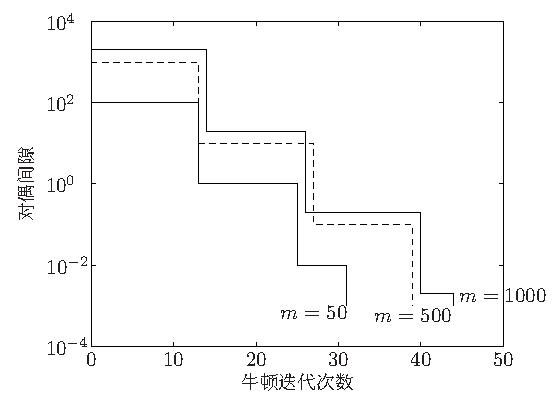
\includegraphics[width=.67\textwidth]{figures/ch11-07.pdf}
\caption*{图11.7 三个不同维数的随机标准形式 LP 的障碍法进展：对偶间隙与累计牛顿步数的关系。各问题变量数为 $n=2m$。这里同样可见对偶间隙近似线性收敛，而较大问题所需的牛顿步数略有增加。}
\end{figure}
\begin{figure}[htbp]\centering
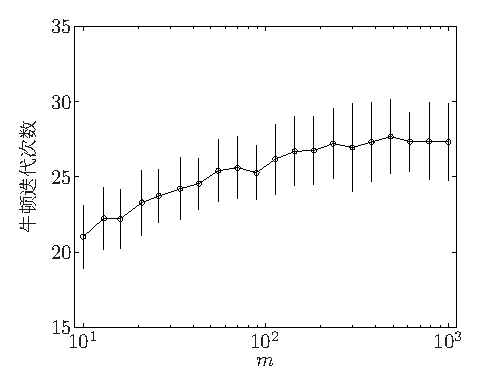
\includegraphics[width=.6\textwidth]{figures/ch11-08.pdf}
\caption*{图11.8 不同维数下求解 $100$ 个随机 LP 所需的平均牛顿步数，$n=2m$。误差棒给出每个 $m$ 值下围绕均值的标准差。问题维数变化 $100$ 倍时，所需牛顿步数的增长很小。}
\end{figure}

% Source PDF page 591 (printed p. 577)
\subsection{收敛性分析}
障碍法的收敛性分析很直接。假设对 $t=t^{(0)},\mu t^{(0)},\mu^2t^{(0)},\ldots$，都能用牛顿法最小化 $tf_0+\phi$，则完成初始中心化以及另外 $k$ 次中心化之后，对偶间隙为 $m/(\mu^k t^{(0)})$。因此，达到要求的精度 $\epsilon$，恰好需要初始中心化，再加上
\begin{equation}
\left\lceil\frac{\log(m/(\epsilon t^{(0)}))}{\log\mu}\right\rceil\tag{11.13}
\end{equation}
次中心化。

因此，只要在 $t\ge t^{(0)}$ 时可以用牛顿法求解中心化问题 (11.6)，障碍法就有效。对于标准牛顿法，一个充分条件是：对 $t\ge t^{(0)}$，函数 $tf_0+\phi$ 满足第10.2.4节（第529页）的条件，即初始下水平集为闭集，相应 KKT 矩阵的逆有界，而且 Hessian 矩阵满足 Lipschitz 条件。（第11.5节将详细讨论基于自协调性的另一组充分条件。）若中心化采用不可行初始点牛顿法，则第10.3.3节（第536页）列出的条件足以保证收敛。

假设 $f_0,\ldots,f_m$ 为闭函数，对原问题作简单修改就能保证这些条件成立。在问题中增加约束 $\norm{x}_2^2\le R^2$，可推出对每个 $t\ge0$，$tf_0+\phi$ 都强凸，特别地，中心化步骤中的牛顿法保证收敛（见习题11.4）。

这一分析说明，在合理假设下障碍法确实收敛，但没有回答一个基本问题：随着参数 $t$ 增大，中心化问题是否越来越难，因而需要越来越多次迭代？数值证据表明，对许多不同类型的问题，情况并非如此：即使 $t$ 增大，中心化问题所需的牛顿步数似乎也近似不变。第11.5节将看到，对于满足某些自协调条件的问题，可以解决这个问题。

\subsection{修改后的 KKT 方程的牛顿步}
在障碍法中，牛顿步 $\Delta x_{\mathrm{nt}}$ 及相应对偶变量由下列线性方程给出：
\begin{equation}
\begin{bmatrix}t\nabla^2 f_0(x)+\nabla^2\phi(x)&A^\T\\A&0\end{bmatrix}
\begin{bmatrix}\Delta x_{\mathrm{nt}}\\\nu_{\mathrm{nt}}\end{bmatrix}
=-\begin{bmatrix}t\nabla f_0(x)+\nabla\phi(x)\\0\end{bmatrix}.\tag{11.14}
\end{equation}
本节说明，中心化问题的这些牛顿步可以解释为以一种特定方式直接求解修改后 KKT 方程
\begin{equation}\begin{aligned}
\nabla f_0(x)+\sum_{i=1}^m\lambda_i\nabla f_i(x)+A^\T\nu&=0,\\
-\lambda_i f_i(x)&=1/t,\quad i=1,\ldots,m,\\
Ax&=b
\end{aligned}\tag{11.15}\end{equation}
时得到的牛顿步。

% Source PDF page 592 (printed p. 578)
修改后的 KKT 方程 (11.15) 是关于 $n+p+m$ 个变量 $x,\nu,\lambda$ 的 $n+p+m$ 个非线性方程。求解时，首先用 $\lambda_i=-1/(tf_i(x))$ 消去变量 $\lambda_i$，得到
\begin{equation}
\nabla f_0(x)+\sum_{i=1}^m\frac1{-tf_i(x)}\nabla f_i(x)+A^\T\nu=0,
\qquad Ax=b,\tag{11.16}
\end{equation}
这是关于 $n+p$ 个变量 $x,\nu$ 的 $n+p$ 个方程。

为求解非线性方程组 (11.16) 的牛顿步，对第一个方程中的非线性项作 Taylor 近似。$v$ 很小时有
\begin{align*}
&\nabla f_0(x+v)+\sum_{i=1}^m\frac1{-tf_i(x+v)}\nabla f_i(x+v)\\
&\quad\approx\nabla f_0(x)+\sum_{i=1}^m\frac1{-tf_i(x)}\nabla f_i(x)+\nabla^2 f_0(x)v\\
&\qquad+\sum_{i=1}^m\frac1{-tf_i(x)}\nabla^2 f_i(x)v
+\sum_{i=1}^m\frac1{tf_i(x)^2}\nabla f_i(x)\nabla f_i(x)^\T v.
\end{align*}
用这个 Taylor 近似替换方程 (11.16) 中的非线性项，就得到牛顿步对应的线性方程
\begin{equation}
Hv+A^\T\nu=-g,\qquad Av=0,\tag{11.17}
\end{equation}
其中
\begin{align*}
H&=\nabla^2 f_0(x)+\sum_{i=1}^m\frac1{-tf_i(x)}\nabla^2 f_i(x)
+\sum_{i=1}^m\frac1{tf_i(x)^2}\nabla f_i(x)\nabla f_i(x)^\T,\\
g&=\nabla f_0(x)+\sum_{i=1}^m\frac1{-tf_i(x)}\nabla f_i(x).
\end{align*}
注意到
\[
H=\nabla^2 f_0(x)+(1/t)\nabla^2\phi(x),\qquad
g=\nabla f_0(x)+(1/t)\nabla\phi(x),
\]
因此由 (11.14)，障碍法中心化步骤的牛顿步 $\Delta x_{\mathrm{nt}}$ 与 $\nu_{\mathrm{nt}}$ 满足
\[
tH\Delta x_{\mathrm{nt}}+A^\T\nu_{\mathrm{nt}}=-tg,\qquad A\Delta x_{\mathrm{nt}}=0.
\]
与 (11.17) 比较可得
\[
v=\Delta x_{\mathrm{nt}},\qquad\nu=(1/t)\nu_{\mathrm{nt}}.
\]
这说明，对偶变量经过缩放后，中心化问题 (11.6) 的牛顿步可以解释为求解修改后 KKT 方程 (11.16) 的牛顿步。

这种方法先从修改后的 KKT 方程中消去变量 $\lambda$，再应用牛顿法求解得到的方程组。另一种变体不预先消去 $\lambda$，而是直接对修改后的 KKT 方程应用牛顿法。这样就得到第11.7节讨论的原始—对偶搜索方向。
